\documentclass[11pt]{scrreprt}

\usepackage{graphicx}
\usepackage[utf8]{inputenc}
\usepackage[onehalfspacing]{setspace}
\usepackage[ngerman]{babel} 
\usepackage[utf8]{inputenc}
\usepackage[babel, german=quotes]{csquotes}
\usepackage[ngerman]{babel}
\usepackage{amsmath}
\usepackage{placeins}
\usepackage[backend=bibtex,
style=alphabetic,
]{biblatex}

\addbibresource{sources.bib}

\title{Wie Kartendienste ans Ziel finden}
\date{06. Juli 2020}
\author{Johannes Quast}

\begin{document}
\begin{titlepage}
	\centering
	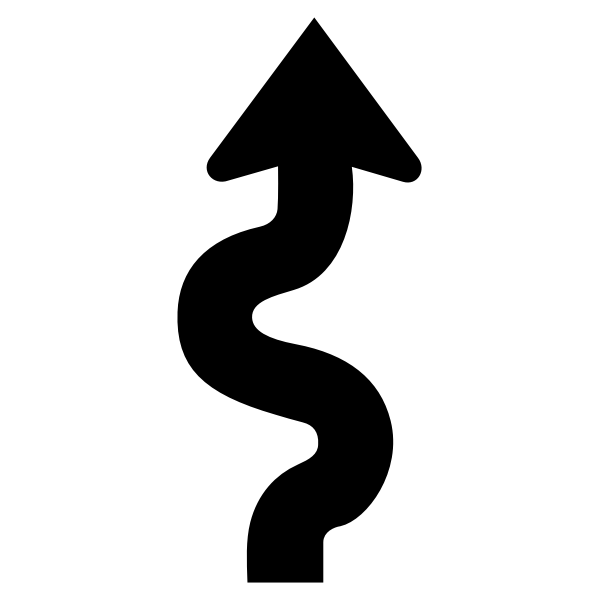
\includegraphics[width=0.33\textwidth]{Bilder/Arrow}\par\vspace{1cm}
	{\scshape\LARGE DHBW Karlsruhe \par}
	\vspace{1cm}
	{\scshape\Large Wissenschaftliches Arbeiten\par}
	\vspace{1.5cm}
	{\huge\bfseries Wie Kartendienste zum Ziel finden\par}
	\vspace{2cm}
	{\Large\itshape Johannes Quast\par}
	
	\vfill
	
	% Bottom of the page
	{\large \today\par}
\end{titlepage}

\tableofcontents

\chapter{Einleitung}
	\section{Motivation}
	Ich glaube jeder von uns kennt die folgende Situation: \\
	Man möchte mit dem Auto oder Verkehrsmittel seiner Wahl an einen bestimmten Ort gelangen, an dem man vorher noch nie gewesen ist.
	Die Lösung dieses Problems heißt heutzutage in den meisten Fällen \enquote{Google Maps} oder trägt den Namen einer anderen populären Kartenapp.
	Kaum hat man eine beliebe Adresse in ein Suchfeld eingegeben, bekommt man bereits nach wenigen Sekunden eine Route vorgeschlagen.
	\\\\
	In Zeiten der Digitalisierung, in der solche Apps für uns selbstverständlich geworden sind und klassische Navigationsmethoden wie z.B. Atlanten oder Karten des Straßennetzes beinahe ausgestorben sind, fragt sich kaum jemand, wie solche Routenplaner eigentlich funktionieren.
	In dieser Ausarbeitung möchte ich genau auf diese Hintergründe eingehen und versuchen \textbf{möglichst anschaulich} zu erklären, wie eine solche Routenberechnung eigentlich funktioniert und welche einfachen Möglichkeiten es gibt, in großen Straßennetzen zu navigieren.

	\section{Vorwort}
	Bevor man sich mit der Routenplanung in einem Straßennetz im speziellen beschäftigt, sollte man dieses Problem auf ein etwas allgemeineres reduzieren: Die Wegfindung von einem Punkt X zu einem Punkt Y.
	Es sollte natürlich selbsterklärend sein, dass Punkt X und Y meistens keine direkte Verbindung zueinander haben, sondern die Route über zahllose Zwischenpunkte gehen wird.
	\\\\
	Um dieses Problem zu lösen gibt es sehr viele Ansätze, aber nicht alle sind praktikabel aufgrund verschiedener Limitationen der jeweiligen Ansätze.
	Auf den folgenden Seiten werden wir einige Möglichkeiten betrachten, sodass am Ende klar sein sollte, welche Möglichkeiten für eine Routenplanung in einem Straßennetz in Frage kommen.

\chapter{Grundlagen}
	\section{Graphen}
	Fast genauso wichtig wie das Verständnis für den Algorithmus ist ein grober Überblick darüber, auf welchen Daten bzw. Datenstrukturen unser Algorithmus arbeiten wird.
	Die Datenstruktur, die für diesen Anwendungszweck in Frage kommt nennt sich \textit{Graph}.
	Vereinfacht gesagt besteht ein Graph aus Knoten (z.B. Punkt X oder Y) und Kanten (Verbindungen zwischen den Knoten). \cite{wiki:german:graphs}

	\begin{figure}[ht]
		\centering
		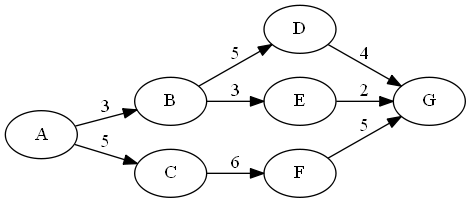
\includegraphics[width=0.7\textwidth]{Graphs/hello}
		\caption{Ein einfacher Graph mit Knoten (A,B,C,...) und Kanten}
	\end{figure}

	Wie man in der Abbildung sehen kann, sind alle Kanten zusätzlich mit Zahlen versehen. Diese geben meistens eine Art \textit{Gewichtung} o.ä. an. Im Kontext der Wegfindung können diese Zahlen zum Beispiel den Aufwand angeben, den jemand benötigt um z.B. von Punkt A zu B zu gelangen. In der realen Welt kann dieser Aufwand beispielsweise mit der Länge der Strecke oder Fahrzeit verbunden werden.
	\newpage

	\section{Prioritätenliste (priority queue)}
	Diese Datenstruktur ist wichtig für viele Algorithmen, die den kürzesten Weg finden möchten.
	Wie der Name bereits vermuten lässt, handelt es sich hierbei um eine Warteschlange, die bestimmte Objekte speichern kann.
	Diese werden nach einer bestimmten \textit{Priorität} geordnet.

	\begin{figure}[ht]
		\centering
		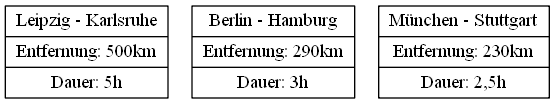
\includegraphics[width=0.8\textwidth]{Graphs/pq_objects}
		\caption{Objekte mit Fahrzeit und Entfernung zwischen zwei Städten}
	\end{figure}
	
	Würde man diese 3 Objekte nun nacheinander in eine Prioritätenliste einfügen, dann würden diese sich automatisch an die richtige Position in der Liste einreihen.
	
	\begin{figure}[ht]
		\centering
		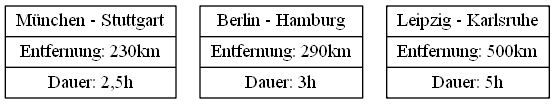
\includegraphics[width=0.8\textwidth]{Graphs/pq_sorted_distance}
		\caption{Objekte in Prioritätenliste: Niedrigere Entfernung = höhere Priorität}
	\end{figure}

\chapter{Algorithmen}
Auf den folgenden Seiten möchte ich mich auf zwei sehr bekannte Algorithmen beschränken, da diese ein sehr gutes Verständnis dafür liefern, wie eine Routenberechnung implementiert werden kann und wie die Wegfindung vorgeht.

	\section{Dijkstra}
	Der erste ist der Dijkstra Algorithmus, auf dem auch A* basiert.
	Er arbeitet auf einem Graphen, um die kürzeste Route zwischen einem gegebenen Startknoten und einem bestimmten Zielknoten zu ermitteln. Jede Kante im Graphen muss dabei eine nicht negative Gewichtung aufweisen.
	

		\subsection{Allgemeine Funktionsweise}
		\begin{enumerate}
			\item Bevor die eigentliche Wegfindung beginnt, wird die Datenstruktur initialisiert. Dabei wird jedem Knoten in unserem Graphen folgende zwei Eigenschaften zugeordnet: Entfernung und Vorgänger. Die Entfernung gibt dabei die Distanz zum Startknoten an. Es ist an dieser Stelle zu erwähnen, dass der Begriff \enquote{Entfernung} hier stark von der verwendeten Kantengewichtung abhängt, denn nicht immer ist die Einheit dieser Werte ein Weg o.ä.
			Alle Knoten haben eine initiale Entfernung von $\infty$, da am Anfang der Suche noch nicht sichergestellt ist, ob ein bestimmter Knoten vom Startknoten überhaupt erreichbar ist.
			Der Startknoten selbst bekommt die Entfernung 0 zugeordnet. \cite{wiki:german:dijkstra}
			
			\item In diesem und den folgenden Schritten kommt die zuvor erklärte \textit{Prioritätenliste} zum Einsatz. Alle Knoten werden in dieser Liste gespeichert und aufsteigend nach der Entfernung sortiert.
			
			\begin{enumerate} 
				\item Nun beginnt man, für alle Nachbarknoten des aktiven Knotens (am Anfang ist dies der Startknoten) die Entfernungen zu berechnen. 
				\begin{equation*}
					Enterfnung_{Knoten_{Nachbar}} = Enterfnung_{Knoten_{Aktiv}} + Kantengewicht
				\end{equation*}
				Diese berechnete Entfernung wird nur gesetzt, wenn die bereits gesetzte Entfernung des Nachbarknotens größer als die neue ist. Sollte dies der Fall sein, wird dieser Wert aktualisiert und das Attribut \textit{Vorgänger} wird auf den aktiven Knoten gesetzt.
				\cite{wiki:german:dijkstra}
				\item Der momentan aktive Knoten wird nun der Liste der \textit{besuchten Knoten} hinzugefügt. Dies hat den einfachen Hintergrund, dass der Algorithmus nicht mehrmals den selben Knoten untersucht, oder ein Zirkel entsteht (z.B. wenn der Algorithmus auf einen Kreisverkehr trifft).
				\item Jetzt beginnt die Schleife erneut bei Schritt a. Allerdings mit dem wichtigen Unterschied, dass der aktive Knoten mit dem ersten Knoten aus der \textit{Prioritätenliste} ersetzt wird. \cite{wiki:german:dijkstra} Kurz zur Erinnerung: Der 1. Knoten dieser Warteschlange ist der Knoten, der momentan die geringste Entfernung zum Startknoten ausweist. Die Schleife \textbf{terminiert}, wenn der aktive Knoten gleich dem gesuchten Zielknoten entspricht.
			\end{enumerate}
			
		\end{enumerate}
	
		\newpage
		\subsection{Beispiel}
		Für das Beispiel verwenden wir den 1. Beispielgraphen. Der Startknoten in diesem Fall ist \textit{A}, der Zielknoten \textit{G}. Der momentan aktive Knoten wird blau markiert, die bereits besuchten Lila. Orange sind die Nachbarknoten, für die gerade die Entfernung berechnet wurde (Vergleich Schritt c. der allgemeinen Funktionsweise).
		Weiterhin werden die Einträge der Prioritätenliste visualisiert, indem jeweils der Name des Knoten selbst, die Entfernung zum Startknoten und über welchen Vorgängerknoten man den betrachteten Knoten erreichen kann, dargestellt wird.
			\subsubsection{1. Schritt}
			\begin{figure}[ht]
				\centering
				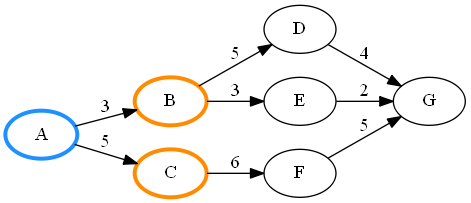
\includegraphics[width=0.8\textwidth]{Graphs/Example1}
				\caption{Graph während Schritt 1: A ist aktiver Knoten, B und C Nachbarknoten}
			\end{figure}
			\begin{figure}[ht!]
				\centering
				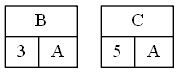
\includegraphics[width=0.3\textwidth]{Graphs/Example1_PQ}
				\caption{Prioritätenliste nach Schritt 1}
			\end{figure}
			Der Knoten A ist in diesem Fall der Startknoten und hat die Nachbarknoten B und C.
			Für beide Nachbarn wird nun die Entfernung berechnet, ausgehend von A.
			\begin{align*}
					Entfernung_B &= Entfernung_A + 3 = 0 + 3 = 3\\
					Entfernung_C &= Entfernung_A + 5 = 0 + 5 = 5
			\end{align*}
			
			\newpage
			\subsubsection{2. Schritt}
			\begin{figure}[ht]
				\centering
				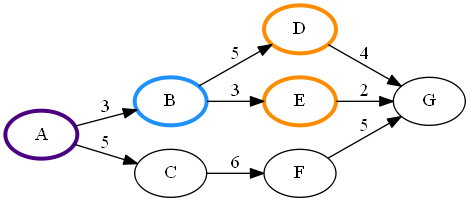
\includegraphics[width=0.8\textwidth]{Graphs/Example2}
				\caption{B ist aktiver Knoten. Für D und E wird Entfernung berechnet. A bereits betrachtet.}
			\end{figure}
			\begin{figure}[ht]
				\centering
				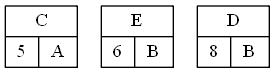
\includegraphics[width=0.45\textwidth]{Graphs/Example2_PQ}
				\caption{Prioritätenliste nach Schritt 2}
			\end{figure}
			\FloatBarrier
			Da der Knoten B in der Prioritätenliste nach Schritt 1. der erste war, wurden die Schritte nun bei diesem wiederholt.
			\begin{align*}
			Entfernung_D &= Entfernung_B + 5 = 3 + 3 = 6\\
			Entfernung_E &= Entfernung_B + 5 = 3 + 5 = 8
			\end{align*}
			
			\newpage
			\subsubsection{3. Schritt}
			\begin{figure}[ht]
				\centering
				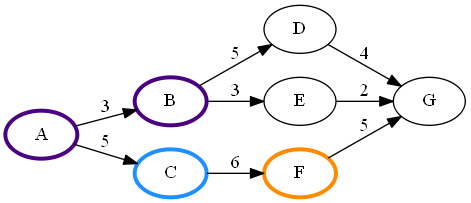
\includegraphics[width=0.8\textwidth]{Graphs/Example3}
				\caption{C ist aktiver Knoten. F wird berechnet. A und B bereits betrachtet}
			\end{figure}
			\begin{figure}[ht]
				\centering
				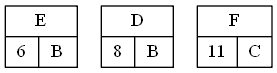
\includegraphics[width=0.45\textwidth]{Graphs/Example3_PQ}
				\caption{Prioritätenliste nach Schritt 3}
			\end{figure}
			\FloatBarrier
			Obwohl C die höchste Anfangsdistanz zum Startknoten aufweist, ist er in der Gesamtdistanz zu A nach dem 2. Schritt an die erste Stelle der Prioritätenliste gerutscht, da der Algorithmus mit den gegebenen Daten nicht wissen kann, dass der Graph sowohl zwischen C und F, als auch zwischen F und G sehr hohe Werte für die Gewichtung aufweist.
			\begin{align*}
			Entfernung_F &= Entfernung_C + 6 = 5 + 6 = 11
			\end{align*}
			
			\newpage
			\subsubsection{4. Schritt}
			\begin{figure}[ht]
				\centering
				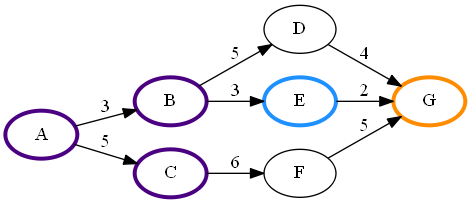
\includegraphics[width=0.8\textwidth]{Graphs/Example4}
				\caption{E ist aktiver Knoten. G wird berechnet. A, B, C bereits betrachtet.}
			\end{figure}
			\FloatBarrier
			Für diesen letzten Schritt stand der Knoten E als erster in der Prioritätenliste. In diesem Fall hat E nur einen Nachbarknoten: den Zielknoten G.
			An diesem Punkt bricht die Schleife ab, nachdem die Entfernung und der Vorgänger bei G gesetzt worden sind.
			\begin{align*}
			Entfernung_G &= Entfernung_E + 2 = 6 + 2 = 8
			\end{align*}
			Über genau diese Vorgängerbeziehung zwischen den Knoten kann man nun den kürzesten Weg rekonstruieren.
			In diesem Beispiel wäre der kürzeste Pfad A $\rightarrow$ B $\rightarrow$ E $\rightarrow$ G.
		
			\begin{figure}[ht]
				\centering
				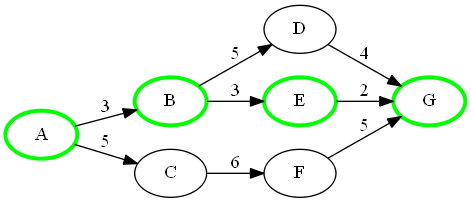
\includegraphics[width=0.8\textwidth]{Graphs/ExamplePathFull}
				\caption{Kürzester Pfad}
			\end{figure}
			\FloatBarrier
			
			\newpage
			Würde man den Pfad über die Beziehungen selbst darstellen, würde dies folgendermaßen aussehen.
			
			\begin{figure}[ht]
				\centering
				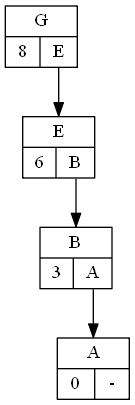
\includegraphics[width=0.2\textwidth]{Graphs/ExamplePath}
				\caption{Kürzester Pfad über Vorgängerbeziehung}
			\end{figure}
			\FloatBarrier
\newpage
\section{A*}
\subsection{Problemstellung}
\begin{figure}[ht]
	\centering
	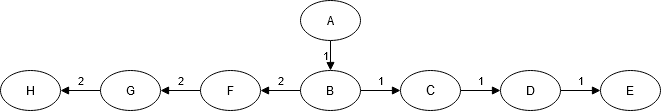
\includegraphics[width=1\textwidth]{Graphs/ExampleHighway}
	\caption{Veranschaulichung einer Kreuzung mit zwei abgehenden Straßen}
\end{figure}
\FloatBarrier
Die Kreuzung aus Abbildung 3.10 besitzt von A kommend zwei abgehende Straßen.
Die nach rechts führenden Streckenabschnitte besitzen alle eine Gewichtung von eins, da in diesem Szenario keine Behinderung für Verkehrsteilnehmer vorliegt. 
Die nach links führenden Streckenabschnitte weisen in diesem Fall einen leichten Stau auf und besitzen deshalb einen Gewichtung von zwei (höherer Aufwand um die Strecke zu befahren). \cite{youtube:english:dijkstra}
Der Startknoten ist A, der Zielknoten H.
\\\\
Wendet man nun Dijkstra auf diesen Graphen an, dann wird man schnell feststellen, dass der Algorithmus den rechten Streckenabschnitten eher nachgehen wird, da dort jede Kante eine geringere Gewichtung aufweist, obwohl der Zielknoten in der genau entgegengesetzten Richtung liegt.
Dieses Verhalten lässt sich dadurch erklären, dass Dijkstra nur die Entfernung zum Startknoten verwendet, um den Graphen zu durchsuchen, aber der Algorithmus dadurch kein Verständnis für Richtungen aufweist.

\subsection{Funktionsweise}
Um genau dieses Problem von Dijkstra zu lösen, verwendet der A* Algorithmus einen leicht anderen Ansatz.
In der Prioritätenliste von A* wird als Priorität statt der Entfernung vom Startknoten (wie bei Dijkstra) folgende Heuristik verwendet. \cite{wiki:german:astar}
\begin{equation*}
	f(x) = g(x) + h(x)
\end{equation*}
$g(x)$ ist die Entfernung des betrachteten Knotens vom Startknoten aus.
Dieser Teil der Heuristik ist genau die Gewichtung, die auch Dijkstra verwendet. \cite{wiki:german:astar}\\\\
$h(x)$ ist der Bestandteil, den A* zur Berechnung hinzufügt. Diese Funktion gibt die eine \textit{Schätzung} an, wie viel es, ausgehend vom betrachteten Knoten im günstigsten Fall \enquote{kostet}, um zum Ziel zu gelangen.\cite{wiki:german:astar}\\\\
$f(x)$ wird dem betrachteten Knoten zugeordnet und die gibt die \textit{Gesamtkosten} an, um zum Ziel zu gelangen, wenn der Pfad durch den betrachteten Knoten verläuft. \cite{wiki:german:astar}
\\\\
Setzt man $h(x)$ auf 0, dann verhält sich A* gleich dem Dijkstra Algorithmus.
Für eine Routenfindung verwendet man häufig als $h(x)$ die Luftlinie zwischen dem betrachteten Knoten und dem Zielknoten.
\\\\
Benutzt man nun für das Beispiel der Problemstellung statt dem Dijkstra den A* Algorithmus mit einer Luftlinie als Heuristik \cite{wiki:german:astar}, dann würden die $h(x)$ für die Knoten des rechten Streckenabschnitts ansteigen und damit die Gesamtkosten, während die Schätzung für den linken Abschnitt immer kleiner wird. Somit umgeht man das beschriebe Problem für dieses konkrete Beispiel.

\chapter{Mögliche Verbesserung}
Die vorherigen Beispiele für die Routenberechnung waren in der Anzahl ihrer Knoten sehr begrenzt.
Schaut man sich nun allerdings ein typisches Alltagsszenario an, dann wird schnell klar, dass ein solcher Algorithmus normalerweise auf einem Graphen mit tausenden Knoten arbeiten wird (z.B. Navigation in Großstädten oder größere Entfernungen).
\\\\
In einem großen Straßennetz wie z.B. von Deutschland, wäre es eine Möglichkeit bei der Routenfindung über größere Distanzen, Autobahnen normalen Landstraßen der Bundesstraßen zu bevorzugen, da man so meistens deutlich schneller ans Ziel gelangt.
\\\\
Auch könnte man eine Art Vorverarbeitung des Graphen vornehmen, indem man sehr wenig befahrene Straßen (z.B. Feldwege) von vornherein nicht berücksichtigt.
\\\\
Weiterhin helfen zusätzliche Daten wie z.B. Geschwindigkeitslimits, Echtzeit Verkehrsdaten oder statistische Auswertung des Verkehrs zu bestimmten Wochentagen/Uhrzeiten bei der Wahl der schnellsten Route, da sich der Verkehr ständig verändert.

\chapter{Fazit}
A* und Dijkstra sind zwei sehr prominente und vielseitig einsetzbare Algorithmen für die Wegfindung in verschiedensten Situation.
Natürlich gibt es noch weitere Algorithmen, die allerdings hier nicht weiter betrachtet wurden und ihre eigenen individuellen Stärken und Schwächen besitzen.
Besonders in Situationen in denen ein Verständnis von \textit{Richtungen} sehr wichtig ist, wie z.B. bei typischen Wegfindungen in Straßennetzen, eignet sich A* hervorragend.
In anderen Anwendungsbereichen in denen dieses Kriterium keine hohe Priorität hat oder die Daten für eine solche Heuristik fehlen, ist Dijkstra die bessere Alternative.

\printbibliography 

\end{document}
